\chapter{Inleiding}
\label{ch:inleiding}

\section{Context}
\label{sec:context}

WiSEO, een bedrijf gespecialiseerd in SEO, had als doelstelling om een onderzoek te doen naar de goedkoopste SEO-tools die aan vooropgestelde eisen voldoen. De bedoeling was om deze tools te gaan vergelijken op basis van een aantal aspecten (zoals prijs en welke informatie ze uiteindelijk leveren) om zo uit te maken welke tools ze zelf zouden gebruiken ter vervanging van of samen met de huidige tools. Van dat onderzoek zal een overzicht gemaakt worden met de functionaliteiten van elke tool. 

Om ervoor te zorgen dat je eigen website of een site van een klant beter scoort in de zoekmachine ben je genoodzaakt om SEO te gaan toepassen. SEO betekent ‘Search Engine Optimization’ of zoekmachineoptimalisatie. Dit is het optimaliseren van een website door het verbeteren van de content, technische aspecten en autoriteit (door meer links te krijgen vanaf andere websites naar je eigen website) met het specifieke doel om beter te scoren bij zoekmachines. ‘Beter scoren’ betekent hier een website hoger krijgen in de zoekresultaten voor relevante zoekwoorden. Zoals je bijvoorbeeld voor een zoekterm ‘wat is seo’ (als seo bedrijf) bovenaan terug te vinden bent: 

\begin{figure}[h!]
\centering
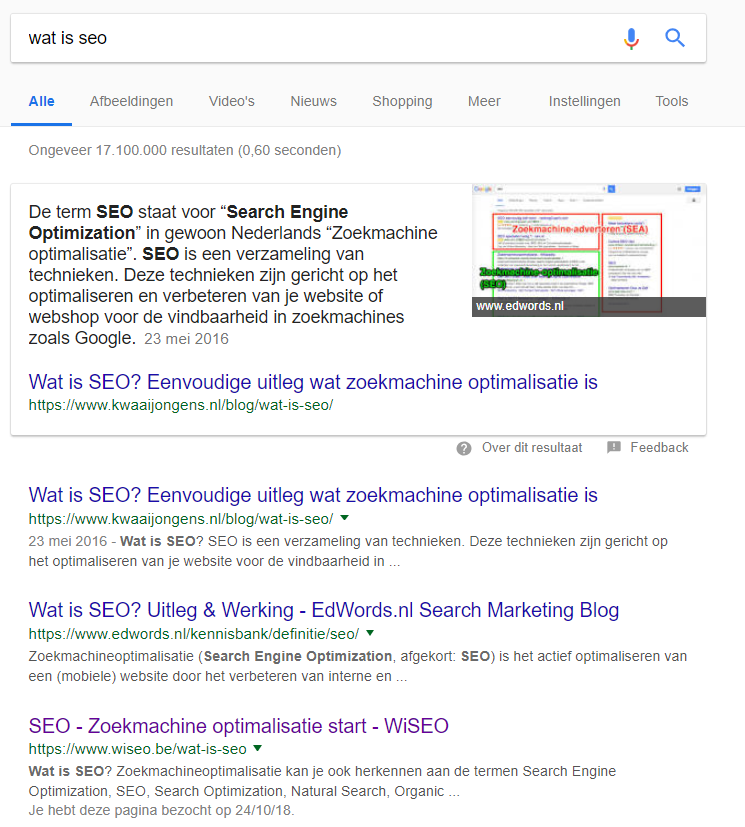
\includegraphics[width=\linewidth]{img/watisseo.png}
\caption{Een afbeelding die een screenshot van de zoekresultaten in Google voor het zoekwoord 'wat is seo' \autocite{google.be}}
\end{figure}

Er zijn bestaan meerdere zoekmachines zoals Bing en Yahoo! maar de meest gebruikte is Google. In dit onderzoek wordt dan ook uitsluitend gewerkt met Google omdat ze meer dan 92\% van het marktaandeel in handen hebben en de focus van WiSEO ook bij Google ligt. Bing en Yahoo! hebben maar elk iets meer dan 5\% marktaandeel samen (op 10/12/2018),          
\textcite{ZOEKMACHINES} .

SEO gaat altijd gepaard met het gebruik van allerlei tools. Deze tools helpen sterk bij: 
\begin{itemize}
\item Het vinden van de juiste zoekwoorden waarop een website moet scoren.
\item Het bekijken van de concurrentie in dezelfde sector of niche.
\item Het controleren alle technische SEO-aspecten op een website.
\item Het vinden van potentiële backlinks (een verwijzing van een andere webpagina naar de eigen site door middel van een link) en zo hoger in de zoekmachine resultaten te komen door autoriteit op te bouwen. Hoe meer inkomende links naar je eigen website, hoe meer dat Google je website als ‘belangrijk’ aanziet. 
\end{itemize}

Kortom, het is bijna onmogelijk om een website te optimaliseren zonder tools te gebruiken voor deze verschillende aspecten.

Op dit moment is er nog geen compleet onderzoek gedaan naar een vergelijking tussen SEO-tools en het resultaat dat ze opleveren. De reden dat dit moet worden onderzocht is omdat WiSEO hierdoor de opdrachten voor middelgrote bedrijven beter kan uitvoeren door middel van een beter zoekwoordenonderzoek, beter concurrentieonderzoek… met als eindresultaat een hogere score in de zoekresultaten.

Het onderzoek bestaat uit 2 delen. Aan de ene kant bestaat het uit een literatuurstudie waar verschillende tools met elkaar vergeleken worden door verschillende aspecten zoals prijs, soort tool en welke gegevens ze opleveren (en dus welke functionaliteiten ze bevatten). Anderzijds wordt een technische uitwerking voorzien door het verbeteren van een SEO-keyword tool. De tool wordt helemaal van nul geprogrammeerd maar een deel van de werking blijft hetzelfde als een tool die al bestaat. 


\section{Stand van zaken in het onderzoeksdomein}
\label{sec:Stand van zaken in het onderzoeksdomein}

In dit onderzoeksdomein zijn er al dergelijke onderzoeken uitgevoerd die vaak in de vorm van blogartikelen terug te vinden zijn. Veel van deze artikelen bijvoorbeeld geven de beste SEO-tools \textcite{SEO13} weer of een volledige lijst van SEO-tools in 2018 \textcite{SEOCOMPLETE}. Ze hebben relevantie tot het onderzoek dat hier gevoerd wordt in de zin dat er ook een vergelijking zal gebeuren tussen meerdere SEO-tools. 

Bij vele van deze blog artikelen wordt er wel geen duidelijk onderscheid gemaakt welke informatie je precies verkrijgt bij een bepaalde tool. Er worden veel tools vermeld waar er tijdelijke trials voor zijn maar je dan achteraf maandelijks een bedrag moet neerleggen. De eerste onderzoeksvraag zal duidelijk het verschil maken tussen gratis en betaalde tools. 


\section{Probleemstelling}
\label{sec:probleemstelling}

Vele SEO-tools in deze vermelde blogartikelen zijn tamelijk duur geprijsd (in de literatuurstudie zal duidelijk zijn wat duur is en wat niet) terwijl er betere alternatieven op de markt bestaan. De meeste tools zijn trials die na verloop van tijd betalend zijn en duur kunnen worden, dit wordt vaak niet of weinig vermeld. Andere tools bieden dan een gratis versie aan maar daar staan altijd beperkingen op. 

Bij de literatuurstudie wordt ook aangetoond dat WiSEO veel tijd verliest met zoekwoordonderzoeken doordat ze handmatig keywords in zoekwoordgroepen moet plaatsen met een Spreadsheet. Daarbij zal er gesuggereerd worden waarom er zelf een keyword tool wordt uitgewerkt. Dit zal gebeuren door een bestaande zoekwoord tool te verbeteren. 


\section{Onderzoeksvragen}
\label{sec:onderzoeksvragen}

Dit onderzoek bestaat uit 2 grote delen waar dan ook meteen 2 onderzoeksvragen uit voorkomen. 

De eerste onderzoeksvraag luidt als volgt: “Welke SEO-tools kunnen best als hulpmiddel gebruikt worden voor meer zichtbaarheid in zoekmachines?”. Hierbij zal een vergelijkende studie gebeuren tussen 4 verschillende soorten tools namelijk: 

\begin{itemize}
\item Zoekwoord onderzoek tools: deze tools worden gebruikt om op zoek te gaan naar de juiste zoekwoorden die je moet gebruiken in je SEO-campagne. Daarbij is het de bedoeling om te zorgen voor betere content (met de juiste zoekwoorden) om het bezoek naar de website op belangrijke zoekwoorden vanuit Google te verhogen. 
\item Ranking tools: hierbij kun je makkelijk zien op welke positie bepaalde zoekwoorden staan in Google voor jouw website. Op die manier kun je snel zien welke zoekwoorden hoog scoren en waar niet. 
\item Backlink tools: backlinks gaan over de autoriteit van een website. Hoe meer links een website heeft van andere websites, hoe meer autoriteit en dus een betere score in Google. Met deze tools kun je bekijken hoeveel links een bepaalde website heeft van andere domeinen en ook welke deze precies zijn. Daarnaast geven sommige tools ook een indicatiescore van de waarde van een domein, hoe meer waarde hoe meer autoriteit in Google.
\item Technische tools: deze tools controleren de technische kant van een website. Hierbij wordt onder andere gekeken naar de metagegevens, de hiërarchie van de URL-structuur en de sitemap van een site.  
\end{itemize}

Aan de hand van enkele aspecten wordt er dan uitgemaakt welke tool de duidelijkste informatie oplevert die SEO'ers (WiSEO en andere SEO-bureaus) het best kunnen gebruiken. Deze aspecten zullen allemaal duidelijk worden uitgelegd in de inleiding van de literatuurstudie. Voor elke soort zal ook een prijsvergelijking plaatsvinden. 

De tweede onderzoeksvraag is: “Hoe gebeurt het verbeteren van een keyword tool zodat er vlotter een zoekwoordonderzoek uitgevoerd kan worden?”. Hierbij zal een eigen tool geprogrammeerd worden om aan te tonen dat er nog verbetering mogelijk is bij zoekwoord tools. 

Er zal een keyword tool geprogrammeerd worden in Java met een eigen ontwerp door gebruik te maken van JavaFX Scene Builder. 


\section{Doelstellingen}
\label{sec:doelstellingen}

De rest van deze bachelorproef is als volgt opgebouwd:

In Hoofdstuk~\ref{ch:studie} wordt er een oplijsting  weergegeven van verscheidene tools. Daarbij zal het duidelijk zijn welke tools best gebruikt kunnen worden per soort tool (zoekwoordonderzoek tools, ranking tools, backlink tools en technische tools) waarbij rekening gehouden wordt met de prijs ervan. De doelstelling is uiteindelijk ook om aan te tonen dat dure tools niet altijd de beste tools zijn en er betere (en goedkopere) alternatieven zijn. 

In Hoofdstuk~\ref{ch:tool} wordt de methodologie toegelicht en worden de gebruikte onderzoekstechnieken besproken om een antwoord te kunnen formuleren op de onderzoeksvragen.

% TODO: Vul hier aan voor je eigen hoofstukken, één of twee zinnen per hoofdstuk

In Hoofdstuk~\ref{ch:conclusie}, tenslotte, wordt de conclusie gegeven en een antwoord geformuleerd op de onderzoeksvragen. 

